Sketch a scatterplot of the data and draw the best-fit line and interpret the picture in context of your answer in (d).

\nl \textbf{Solution: } Look at this photograph:
\notab{
    \begin{center}
        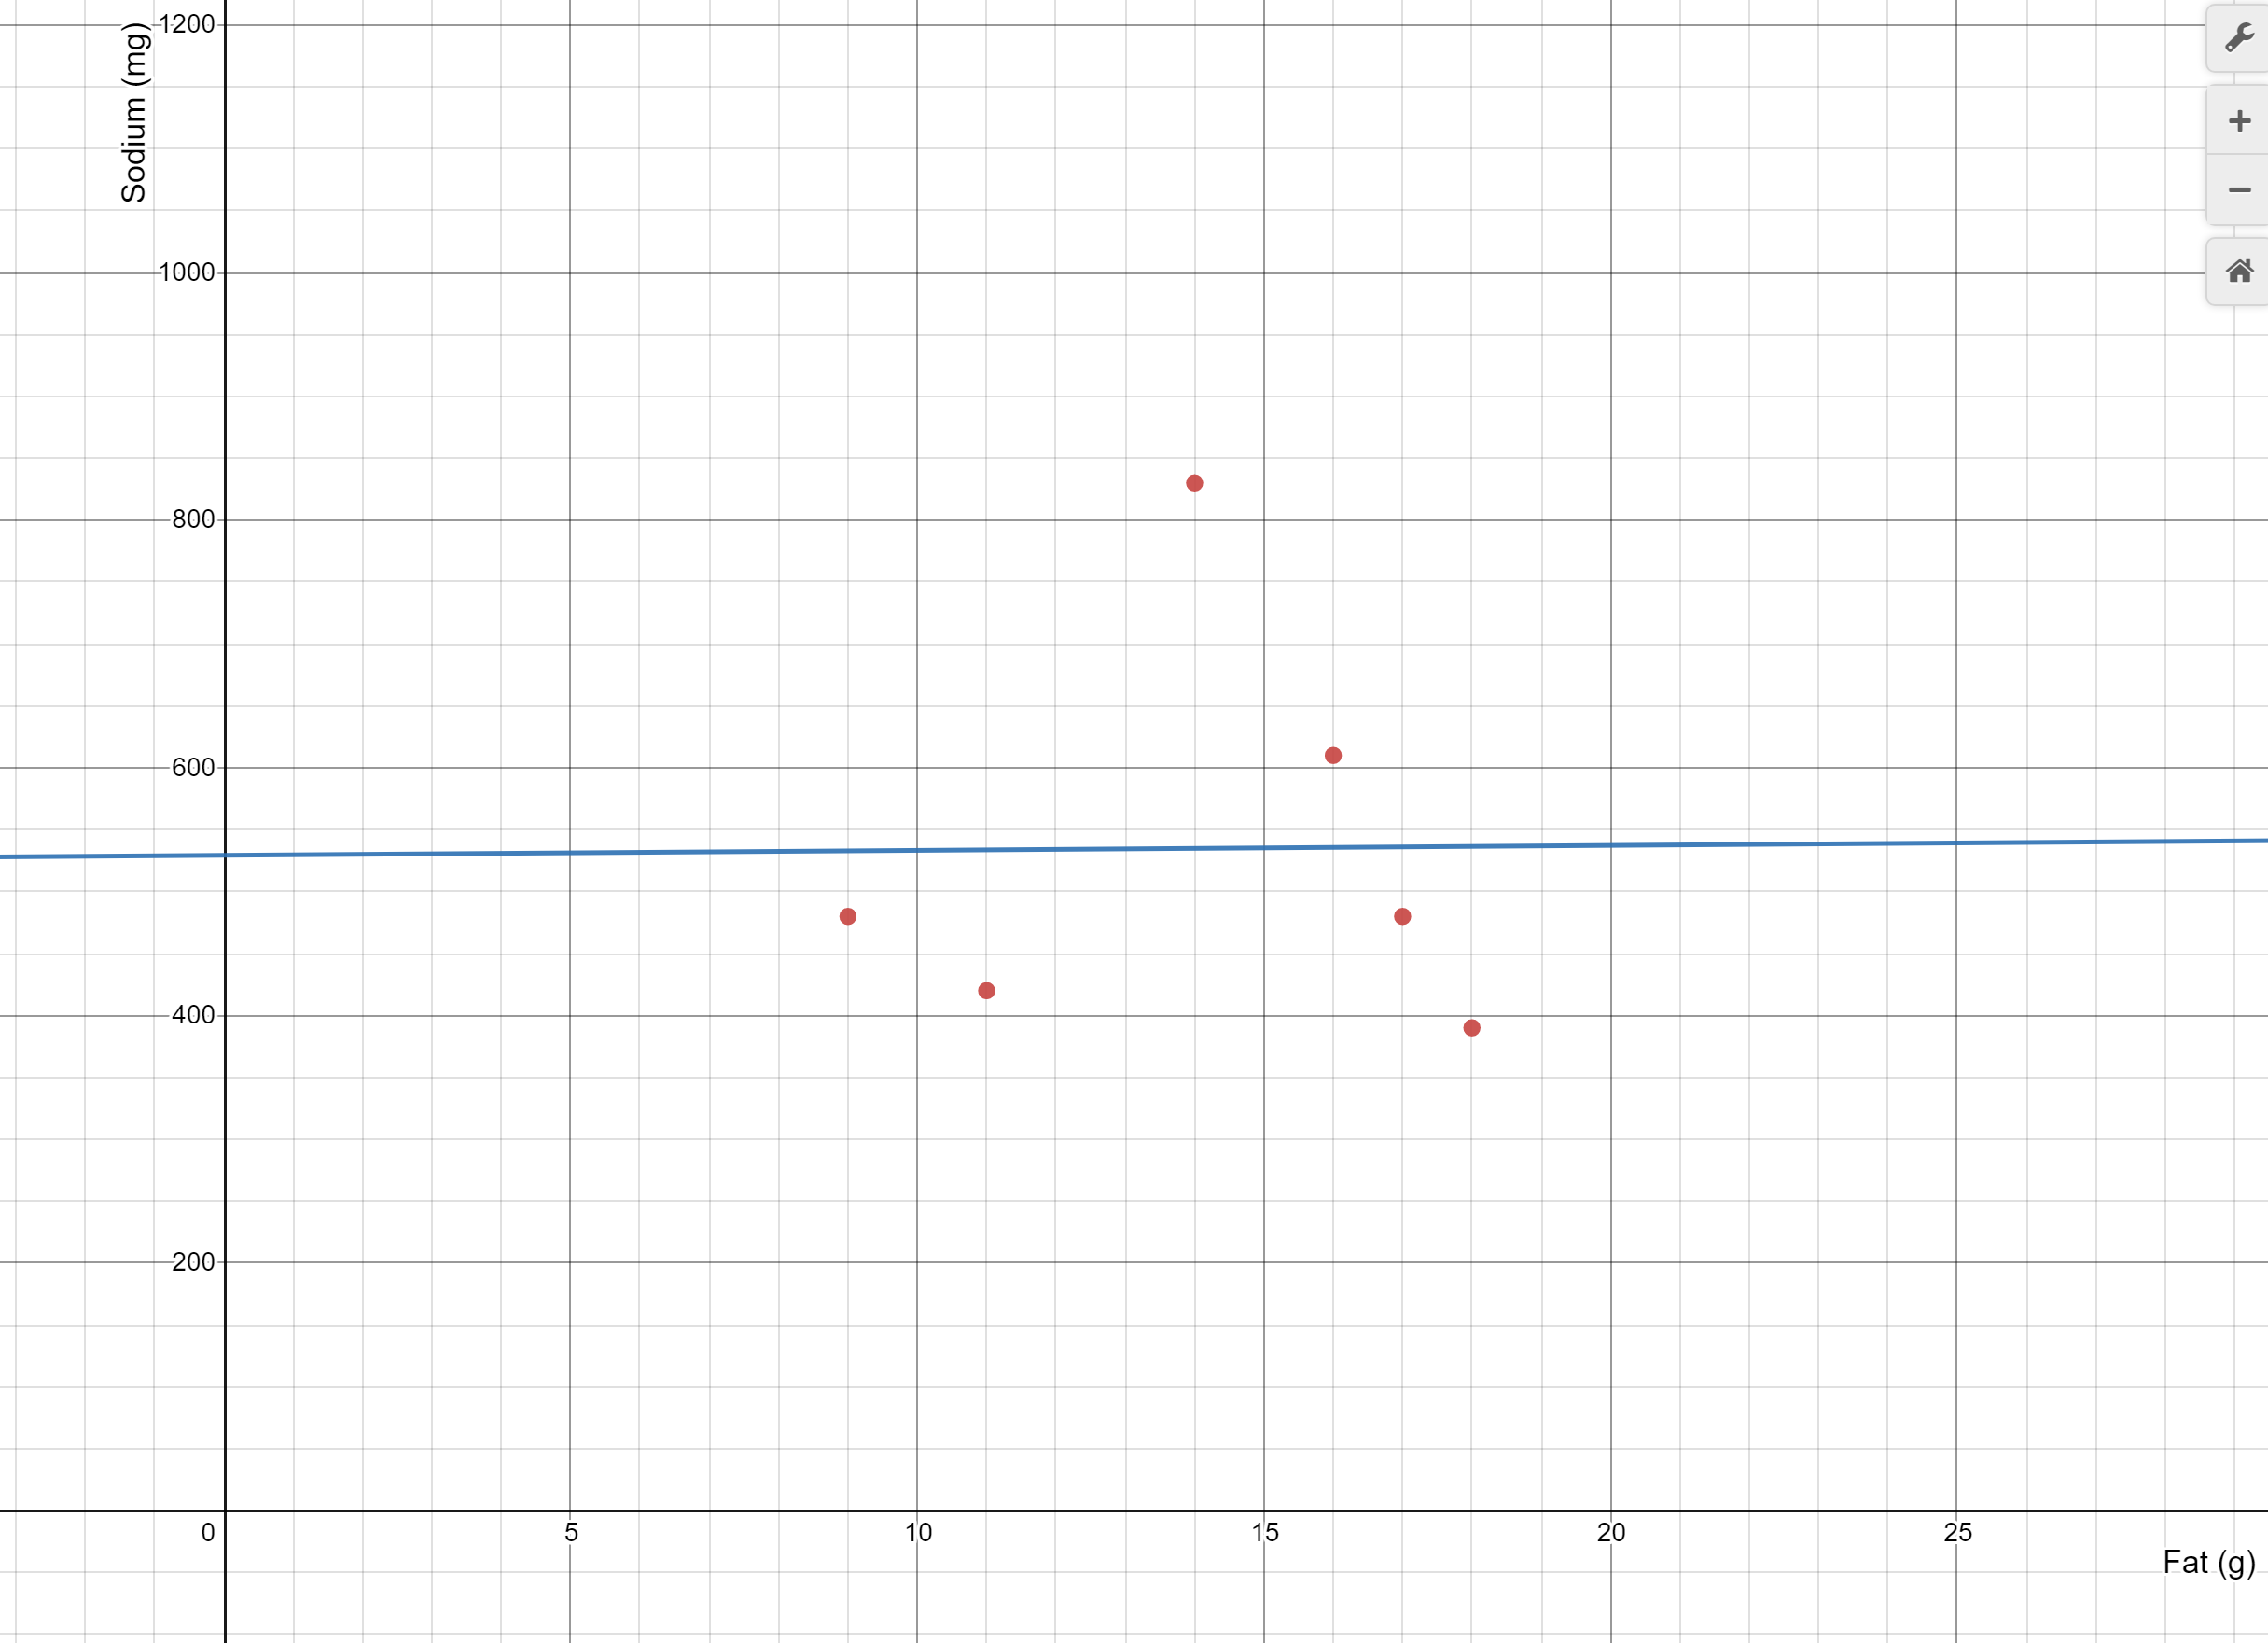
\includegraphics[width=6.75in]{graph.png}
    \end{center}
}
Now, the line does not look as terrible. It could be around 1200 on the y-intercept and about 20 on the x-intercept and go between the set of points to be a bit more accurate. If $(11, 420)$ is an outlier, then a quadratic regression could be useful with a maximum around $(14,800)$. The right cluster looks very linear, but there is some weird shear between the 2nd and 3rd points (from left to right). That, or there is just no correlation between these with any regression curve and it is just a coincidence that the right cluster is linear.